\chapter{Theory and phenomenology of the \BdKstee decay}
\chaptermark{Chapter2}
\label{chapter1}
The \BdKstee decay proceeds via a flavour-changing neutral current (FCNC) and is therefore particularly sensitive to contributions from physics beyond the Standard Model (SM). The decay is forbidden at tree-level and will proceed through higher order diagrams. New physics can manifest in the loop and cause deviations from SM predictions.\\
This chapter starts with an introduction to the effective theories used to describe the \BdKstll decays. The first section is followed by an explication of the \bsg transition which is the main contribution to the \BdKstee decay. In the framework of the SM, the photons from the \bsg transition are predicted to be dominantly left-handed and therefore the measurement of a significant right-handed polarisation amplitude would be a sign for new physics.\\
The measurement of the photon polarisation can be performed by an angular analysis of the \BdKstll decay which is explored in Section \ref{sec:ksll}.\\
The advantages of using the electron-final state in \BdKstee at low invariant dilepton mass $q$ are illustrated at the end of this chapter.


\section{Effective Theories and effective Hamiltonian}
The transitions in the \BdKstll decay are carried out by the weak interaction (energy scale $\mu \sim O(m_b)$) while the binding of the quarks to mesons happens by the strong interaction (energy scale $\mu \sim O(1 \gev )$). Therefore the \BdKstll decay is a multi-scale process that can be described using the Effective Field Theories. Due to the strong hierarchy between external and internal scales a mathematical separation between low and high energy terms can be performed within the framework of the Operator Product Expansion (OPE) \cite{buras}.\\
The effective Hamiltonian can then be expressed in terms of effective point-like vertices which are represented by the local operators $\Opei(\mu)$  and their associated Wilson coefficients $\Ci(\mu)$ which can be regarded as coupling constants associated with these effective vertices.
The effective point-like vertices are introduced because Feynman diagrams such as those in Figures \ref{fig:bsg} and \ref{fig:feynbox} with full \W , \Z and \tquark propagators only represent the interaction at very short distance scales ($\mu \sim O(m_W, m_Z, m_t)$) while the long distance operators with scales of $\mu \sim O(m_b)$ have to be taken into account too. The resulting effective Hamiltonian can be expressed as
\vspace*{-0.3cm}
\begin{equation}
\mathcal{H}_{eff} = -\frac{4G_F}{\sqrt{2}}\Vtb \Vts^* \sum_{i=1}^{10} [\Ci(\mu)\Opei(\mu) + \Cpi(\mu)\Opepi(\mu)]\\
\vspace*{-0.4cm}
\label{eq:genhamilton}
\end{equation}
The dashed variables $\Cpi(\mu)$ and $\Opepi(\mu)$ represent the chirality-flipped Wilson coefficients and local operators respectively.\\
Since the energy scale in \B physics is typically chosen to be $\mu \sim O(m_b)$, the local operators $\Opei(\mu \sim O(m_b))$ have to be calculated using non-perturbative methods. The Wilson coefficients on the other hand, are calculated at $\mu \sim O(m_W)$ -- where perturbative techniques can be applied -- up to NNLO (Next to Next to Leading Order). Renormalisation techniques are then applied to find their values at the appropriate energy scales $\mu \sim O(m_b)$.\\

\section{The photon polarisation in the \bsg transition}
The \bsg transition is the main contribution to the \BdKstll decay at low dilepton invariant mass $q$. The corresponding Feynman diagrams are shown in Figure \ref{fig:bsg}.\\  
The process can be expressed in the effective theory by the magnetic-operators $\squarkbar_L \sigma_{\mu \nu} \bquark_R$ and $\squarkbar_R \sigma_{\mu \nu} \bquark_L$ which introduce the helicity structure $\bquark_R \rightarrow \squark_L \g_L $ and \\$\bquark_L \rightarrow \squark_R \g_R $ \cite{emi}. Due to the fact that the \W bosons only couple to fermions of left-handed chirality, the magnetic operators are weighted with the mass of the \bquark quark and \squark quark respectively $m_{\bquark} \squarkbar_L \sigma_{\mu \nu} \bquark_R$ and $m_{\squark} \squarkbar_R \sigma_{\mu \nu} \bquark_L$.\\
As a result, the second process is suppressed by the factor $m_{\squark} / m_{\bquark}$ which means that the photons from the \bsg transition are dominantly left-handed. Expressed in amplitudes of the photon polarisation this yields a suppression factor of $ \frac{A_R}{A_L} \sim \frac{m_{\squark } }{ m_{\bquark } } $ ($A_R$: right-handed polarisation amplitude, $A_L$: left-handed polarisation amplitude). Taking into account additional gluon contributions in the penguin-diagram and QCD corrections, the SM prediction for the ratio of right-handed amplitude to left-handed amplitude is $\frac{A_R}{A_L} \approx 4 \,\% $  \footnote{Assuming no \CP violation in the \bsg, the statements for the \bsg transition are also true for the \CP transformed process. This means that the photons from the \absg transition are dominantly right-handed and $ \frac{ \bar{A} _L}{ \bar{A} _R} \approx 4 \,\% $.}\cite{ananote}. Therefore a measurement of a significant right-handed amplitude is an unambiguous signal for new physics.\\
\begin{figure}[ht]
  \begin{center}
  	\subfigure{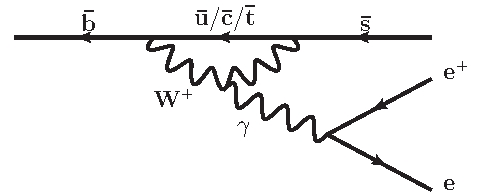
\includegraphics[width=0.45\textwidth]{feynbsg1.jpg}}
   \subfigure{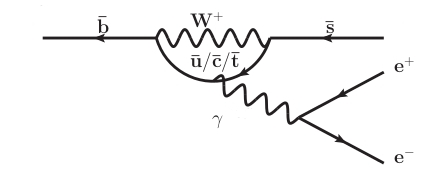
\includegraphics[width=0.49\textwidth]{feynbsg2.jpg}}
  \vspace*{-0.5cm}
  \end{center}
  \caption{\textit{The Feynman diagrams for the \bsg transition.}}
  \label{fig:bsg}
\end{figure}
\newpage
\section{Angular analysis of the \BdKstee}
\label{sec:ksll}
While various ways to measure the photon polarisation have been presented by theorists \cite{ananote} \cite{gross}, the angular analysis of a decay of the form \BdKstll (with $\Kstarz \rightarrow \Kp \pim$) is one of the most promising.\\
This decay proceeds predominantly via the \bsll transition with a virtual photon decaying into two leptons. Since the photon is virtual the kinematics in the \bsll transition are the same as in the \bsg transition, particularly the helicity structure is the same.\\
In \B decays into two vectors (here the virtual photon and the \Kstarz) the subsequent decays of the vectors contain their relative polarisation information \cite{krueger}. Thus, the angular distribution in the relative angles of the $\Kstarz \rightarrow \Kp \pim$ decay plane and the plane of the lepton-pair can be used to determine the helicity amplitudes in the \BdKstll decay and therefore the polarisation amplitudes $A_R$ and ${A_L}$ of the photon.\\

\subsection{Contributions to the \BdKstll Hamiltonian}
The \BdKstll decay proceeds at low lepton-pair invariant mass predominantly via the \bsll transition but other transitions such as the diagram of Figure \ref{fig:bsg} where the photon is replaced by a \Z or the box-diagram in Figure \ref{fig:feynbox} add a non-negligible contribution to the effective Hamiltonian.
\begin{figure}[ht]
\begin{center}
  	\vspace*{-0.5cm}
    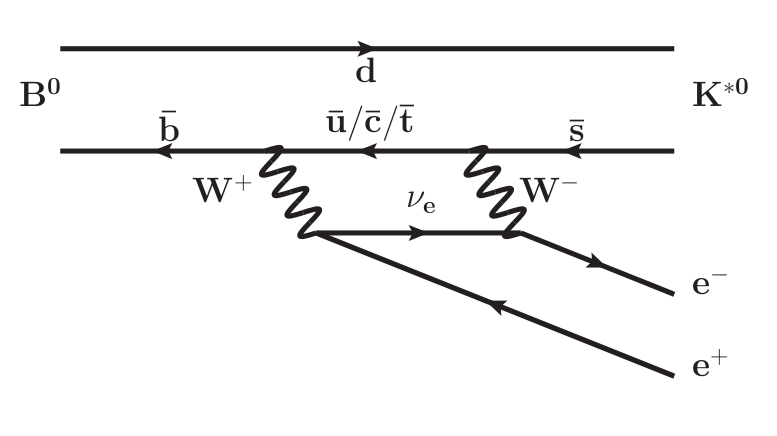
\includegraphics[width=0.48\textwidth]{feynbox.jpg}
  \vspace*{-1cm}
  \end{center}
  \caption{\textit{The box-diagram that contributes to \BdKstll.}}
  \label{fig:feynbox}
\vspace*{-0.5cm}
\end{figure}


The leading order contributions to the \BdKstll effective Hamiltonian (see Equation \ref{eq:genhamilton}) come from the operators $ \Ope7 $ , $ \Ope9 $ and $ \Ope10 $ \cite{krueger}.\\
\begin{eqnarray}
\mathcal{H}_{eff} = -\frac{4G_F }{ \sqrt{2} } \Vtb \Vts^* [& \C7 (\mu) \Ope7 (\mu) + \Cp7 (\mu) \Opep7 (\mu) & \nonumber \\
& \C9 (\mu) \Ope9 (\mu) + \Cp9 (\mu) \Opep9 (\mu) & \ + \ \C10 (\mu) \Ope10 (\mu) + \Cp10 (\mu)\Opep10 (\mu) ]  \nonumber
\label{eq:hamilton}
\end{eqnarray}
with the local operators \cite{gross}
\begin{eqnarray}
& \Ope7 = \frac{e}{16\pi^2} \squarkbar \sigma_{\mu \nu}(m_{\bquark}  P_R \ +\ m_{\squark}P_L)\bquark F^{\mu \nu} &\\
&\Ope9 = \frac{e^2}{16\pi^2} (\squarkbar \gamma_{\mu} P_L \bquark)(\bar{\electron}\gamma^{\mu}\electron) \qquad \Ope10 = \frac{e^2}{16\pi^2} (\squarkbar \gamma_{\mu} P_L \bquark)(\bar{\electron}\gamma^{\mu} \gamma_5 \electron) & \nonumber
\end{eqnarray}

The $ \Ope7 $ corresponds to the SM \bsll transition (\bsg transition) with a left-handed weak-charged current. Since there are no right-handed weak-charged currents in the SM, the $ \Cp7(\mu) $ is only non-zero for contributions from new physics. It is therefore appreciable to measure quantities connected to \Cp7 . 
\\The operators $ \Ope9 $ and $ \Ope10 $ represent the contributions to the \BdKstll decay that do not come from the \bsg transition but for example from the box-diagram in Figure \ref{fig:feynbox}.\\
The branching ratio \BR(\BdKstll) increases significantly towards low $q^2$ values
 (where $q^2$ denotes the square of the dilepton invariant mass)\cite{jaeger}. This is due to the strong increase of the \BR(\bsll) while the other contributions to \BdKstll vary much more smoothly and show no particular increase at low $q^2$. These other contributions make up for a few \% of the events with $20\mevcc < q < 1\gevcc $.\\
At \lhcb the angular analysis of \BdKstll decays is performed with muons and electrons in different bins of $q^2$. The combination of these analyses gives global information about all polarisation amplitudes over a large range of $q^2$ and the relative contributions from $\C9 (\mu)$ and $ \C10 (\mu)$ can be determined. 
\begin{figure}[ht]
  \centering
    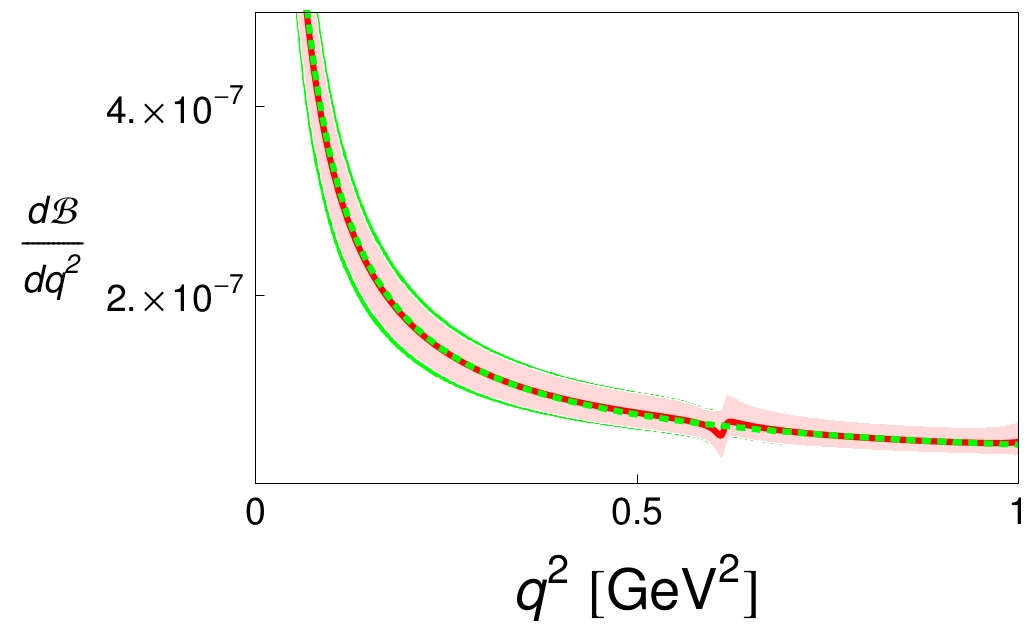
\includegraphics[width=0.55\textwidth]{BR.jpg}
  \caption{\textit{The \BR(\BdKstee) for the low $q^2$ region. Solid (red) and dashed (green) lines correspond to the SM prediction for two different models. The error band is calculated from different theoretical uncertainties such as hadronic and CKM uncertainties and renormalization scale dependence.}\cite{jaeger}}
  \label{fig:BR}
\end{figure}

\subsection{Polarisation amplitudes for the \BdKstee}
\label{sub:polamp}
In the framework of the effective theory, the transversity polarisation amplitudes $A^{L,R}_{ \perp }$, $A^{L,R}_{ \parallel }$ and $A^{L,R}_0$ can be expressed in terms of the Wilson coefficients \cite{krueger}. The indices $L$ and $R$ refer to the chirality of the lepton current. In this calculation the leptons are presumed to be massless which is a very good approximation for the \BdKstee. In the region low $q^2$ region which corresponds to large recoil of the \Kstarz, the amplitudes can be expressed as:
\begin{equation}
A^{L,R}_{ \perp }(q^2) = \frac{ \sqrt{2} N (M^2_B - q^2) }{ M_B }[(\C9 + \Cp9 ) \mp (\C10 + \Cp10 )+\frac{ 2 m_b M_B }{ q^2 } (\C7 + \Cp7 )] \xi_{ \perp }(q^2)
\end{equation}
\begin{equation}
A^{L,R}_{ \parallel }(q^2) = \frac{ \sqrt{2} N (M^2_B - q^2) }{ M_B } [(\C9 + \Cp9 ) \mp (\C10 + \Cp10 )+ \frac{ 2 m_b M_B }{ q^2 }(\C7 - \Cp7 )] \xi_{ \perp }(q^2)
\end{equation}
\begin{equation}
A^{L,R}_0 (q^2) = \frac{ \sqrt{2} N (M^2_B - q^2) }{M_B } [(\C9 + \Cp9 ) \mp (\C10 + \Cp10 )+ \frac{2 m_b }{M_B }(\C7 - \Cp7 )] \xi_{ \parallel }(q^2)
\end{equation}
 
In the above formulae $ \lambda = M_B^4 + M_{\Kstarz}^4 + q^2 - 2(M_B^2 M_{\Kstarz}^2 + M_{\Kstarz}^2 q + M_B^2 q  ) $ and
\begin{equation}
N = \Bigg[ \frac{G_F^2 \alpha^2}{3 \cdot 2^{10}\pi^5 M_B^3} |\Vtb \Vts^* |^2 q \lambda^{1/2} \Big( 1 - \frac{4 m_l^2}{q} \Big)^{1/2} \Bigg]
\end{equation}
and $M_B$: mass of the \B meson, $M_{\Kstarz} $: mass of the \Kstarz meson, $m_b $: mass of the \bquark quark, $m_l $: mass of the lepton. The  $\xi_{ \perp }(q^2)$ and  $\xi_{ \parallel }(q^2)$ factors are the form factors of the \Kstarz meson and contain the non-pertubative physics. As can be seen in those formulae, the polarisation amplitudes are sensitive to new physics that might appear in the Wilson coefficients.\\
Four parameters can be expressed as a combination of the transversity amplitudes and subsequently fitted:
\begin{equation}
F_L(q^2) = \frac{ |A^{L}_0|^2 + |A^{R}_0|^2 }{ |A^{L}_0|^2 + |A^{L}_{ \perp } |^2 + | A^{L}_{ \parallel } |^2 +  |A^{R}_0|^2  + | A^{R}_{ \perp } |^2 + | A^{R}_{ \parallel } |^2 }
\end{equation}
\begin{equation}
A_{FB}(q^2) = \frac{3}{2} \frac{ \Re ( A^L_{ \parallel }( A^L_{ \perp } )^* ) - \Re (A^R_{ \parallel }( A^R_{ \perp } )^* ) }{ | A^L_0 |^2 + | A^L_{ \perp } |^2 + | A^{L}_{ \parallel } |^2 +  | A^{R}_0 |^2  + | A^{R}_{ \perp } |^2 + |A^R_{ \parallel } |^2 }
\end{equation}

\begin{equation}
A^{(2)}_T(q^2) = \frac{|A^{L}_{ \perp }|^2 + |A^{R}_{ \perp }|^2 - |A^{L}_{ \parallel }|^2 - |A^{R}_{ \parallel }|^2 }{|A^{L}_{ \perp }|^2 + |A^{R}_{ \perp }|^2 + |A^{L}_{ \parallel }|^2 + |A^{R}_{ \parallel }|^2}
\end{equation}

\begin{equation}
A^{Im}_T(q^2) = \frac{2 \Im (A^{L}_{ \parallel } (A^{L}_{ \perp })^* + A^{R}_{ \parallel } (A^{R}_{ \perp })^*)}{|A^{L}_{ \perp }|^2 + |A^{R}_{ \perp }|^2 + |A^{L}_{ \parallel }|^2 + |A^{R}_{ \parallel }|^2}
\end{equation}
It can be seen from this formulae that the $A^{(2)}_T(q^2)$ and the $A^{Im}_T(q^2)$ don't depend on the hadronic form factors $\xi_{ \perp }(q^2)$ and $\xi_{ \parallel }(q^2)$ any more, thus a great systematic uncertainty from the theoretical part is removed.\\
The amplitudes for the photon polarisation $A_L$ and $A_R$ can be related to the transversity amplitudes
\begin{equation}
A_{\perp} = \frac{A_R - A_L}{\sqrt{2}} \qquad \qquad  A_{\parallel} = \frac{A_R + A_L}{\sqrt{2}}
\end{equation}
and to $A^{(2)}_T$
\begin{equation}
A^{(2)}_T(q^2) = -2 \Re \Big( \frac{A^*_R(q^2)A_L(q^2)}{|A_R| ^2+ |A_L|^2} \Big) \sim - 2\, \frac{A_R}{A_L}
\end{equation}
The approximation holds up if $\frac{A_R}{A_L}$ is small and real.
%For the low invariant dilepton mass limit $q^2 \rightarrow 0$ the contributions from the Wilson coefficients \Ope9 and \Ope10 become negligible and the amplitude $A^{(2)}_T(q^2)$ can be simplified to
%\begin{equation}
%A^{(2)}_T(q^2 \rightarrow 0) = \frac{2 \Re ( \C7 \, (\Cp7 )^*)}{| \C7 |^2 + | (\Cp7 )^*|^2} = 2\, \frac{A_R}{A_L}
%\end{equation}
This shows clearly that the variable $A^{(2)}_T(q^2)$ is the one that contains the information about the photon polarisation.\\
\newpage
\subsection{Angular distribution}
\label{sec:angles}
The \BdKstll decay is completely defined by four independent kinematic variables; namely the lepton-pair invariant mass $q$ and the three angles $\theta_l$, $\theta_K$ and $\Phi$ which are illustrated in Figure \ref{fig:winkel} \cite{krueger} \cite{ananote}. The angles are defined as:
\begin{itemize}
\item $\theta_l$: the angle between the direction of the vector of the \en (\ep) in the dilepton rest frame, and the direction of the dilepton in the $B^0$ ($\bar{B}^0$) rest frame
\item $\theta_K$: the angle between the direction of the vector of the \pion in the \Kstarz (\Kstarzb) rest frame, and the direction of the \Kstarz (\Kstarzb) in the $B^0$ ($\bar{B}^0$) rest frame
\item $\Phi$: the angle between the planes defined by the \Kstarz daughters and the dileption daughters, in the rest frame of the \B meson.
\end{itemize}

\begin{figure}[!h]
  \begin{center}
  	\vspace*{-0.5cm}
 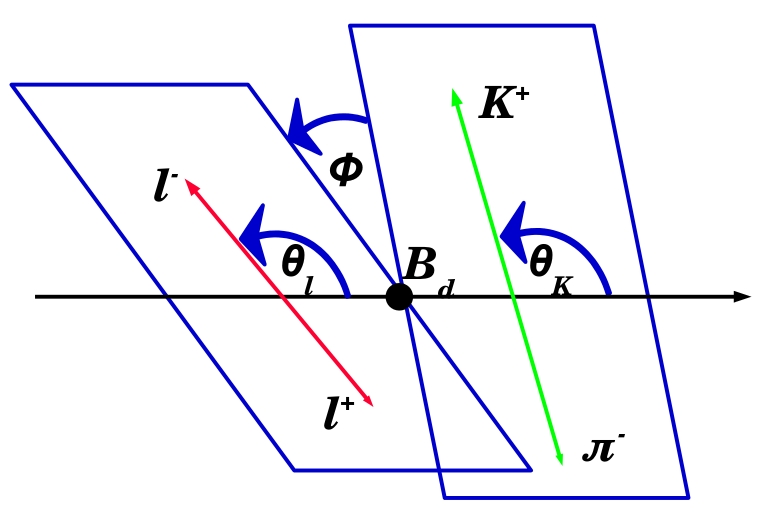
\includegraphics[width=0.6\textwidth]{winkel.jpg}
  \vspace*{-0.8cm}
  \end{center}
  \caption{\textit{Definition of the angles $\theta_l$, $\theta_K$ and $\Phi$ in the \BdKstll decay.}}
  \label{fig:winkel}
\end{figure}

The normalized differential decay width can be expressed as
\begin{equation}
\frac{1}{\Gamma}\frac{d^4 \Gamma}{dq^2 \, \ctl \, \ctk \, d\Phi} = \frac{9}{32 \pi}\sum_{i=1}^{9} I_i'(q^2, \theta_K) f_i(\theta_l , \Phi)
\end{equation}
where the $I_i'$ depend on $q^2$, $\theta_K$ and the helicity polarisation amplitudes $F_L(q^2)$, $A_{FB}(q^2)$, $A^{(2)}_T(q^2)$ and $A^{Im}_T(q^2)$. The $f_i$ are the corresponding angular distribution functions
\begin{eqnarray}
f_1 = 1 \qquad & f_2 = \cos(2\theta_l) \qquad & f_3 = \sin^2(\theta_l) \cos(2\Phi)\nonumber\\
f_4 = \sin(2\theta_l) \cos(\Phi) \qquad & f_5 = \sin(\theta_l) \cos(\Phi) \qquad & f_6 = \cos(\theta_l)\\
f_7 = \sin(\theta_l)\sin(\Phi) \qquad & f_8 = \sin(2\theta_l)\sin(\Phi)\qquad & f_9 = \sin^2(\theta_l)\sin(2\Phi)\nonumber
\end{eqnarray}
The $I_i$ which are sensitive to the ratio of photon polarisations $\frac{A_R}{A_L}$ are $I_3$ and $I_9$. The partial decay width can then be simplified without any loss in information about the photon polarisation by folding the angular distributions for $\Phi$ and $\theta_l$. $\Phi$ is folded by moving all values with $\Phi <0$ to $\Phi + \pi$. This removes the terms proportional to $\cos(\Phi)$ and $\sin(\Phi)$ without affecting the $\cos(2\Phi)$ and $\sin(2\Phi)$ terms. The angle $\theta_l$ is folded by mapping the interval $(\pi /2, \pi)$ onto $(0, \pi /2)$ which removes the term proportional to $\cos(\theta_l)$. 
The decay width after these transformations and neglecting the lepton mass term -- which is legitimate for the \BdKstee decay where $\frac{m^2_{\electron}}{q^2} << 1$ -- is
 \begin{eqnarray}
 \frac{1}{\Gamma}\frac{d^4\, \Gamma}{dq^2 \, \ctl \, \ctk \, d\Phi} = \frac{9}{32 \pi} [  I_1'(q^2, \cos\theta_K)\ +   I_2'(q^2, \cos\theta_K)\, (2\cos^2\theta_l -1) \nonumber \\
  +  I_3'(q^2, \cos\theta_K)\, \sin^2\theta_l \, \cos2\Phi \ +  I_9'(q^2, \cos\theta_K)\, \sin^2\theta_l \, \sin2\Phi ]
 \label{eq:partw}
 \end{eqnarray}
The $I_i'$ terms can be expressed as
\begin{eqnarray}
 I_1'(q^2, \cos\theta_K) &=& \frac{3}{4} (1-F_L(q^2)) \cdot (1-\cos^2\theta_K) + F_L(q^2) \cdot \cos^2\theta_K \nonumber \\
 I_2'(q^2, \cos\theta_K) &=& \frac{1}{4} (1-F_L(q^2)) \cdot (1-\cos^2\theta_K) - F_L(q^2) \cdot \cos^2\theta_K \nonumber \\
 I_3'(q^2, \cos\theta_K) &=& \frac{1}{2} (1-F_L(q^2)) \cdot A^{(2)}_T(q^2) \cdot (1 - \cos^2\theta_K)   \label{eq:is} \\
   I_9'(q^2, \cos\theta_K) &=& \frac{1}{2} (1-F_L(q^2)) \cdot A^{Im}_T(q^2) \cdot (1 - \cos^2\theta_K)  \nonumber 
\end{eqnarray}
By performing an angular analysis, all three remaining parameters $F_L(q^2)$, $A^{(2)}_T(q^2)$ and $A^{Im}_T(q^2)$ can be fitted at the same time and the information about the photon polarisation can be extracted. \\

\subsection{The advantages of the low $q^2$ bin in \BdKstee}
This masters thesis is part of an angular analysis that focusses on the low dilepton invariant mass $q$ region in the \BdKstee decay.\\
The choice of performing the analysis with electrons as opposed to with muons is that the sensitivity to new physics -- which could affect the photon polarisation -- is increased. This is due to the fact that the electron mass is negligible compared to $q^2$: $m^2_e<< q^2$. For a non-negligible lepton mass the $I_3'$ and $I_9'$ in Equations \ref{eq:is} are multiplied by $(1-x)$ with $ x = \frac{4m^2_{l}}{q^2}$ which thus degrades the sensitivity on $A^{(2)}_T(q^2)$ and $A^{Im}_T(q^2)$. In addition the kinematically allowed $q^2$ range is larger.\\
The choice of $20 \mevcc < q < 1\gevcc $ has two distinct advantages. The first advantage is that the contribution coming from the non-\bsll transitions in \Ope9 and \Ope10 are very small (a few \%) and therefore $A^{(2)}_T(q^2) \sim -2\, \frac{A_R}{A_L}$\footnote{Note that the angles in Section \ref{sec:angles} are defined such that for each the \bsll and the \bbsll decay $A^{(2)}_T(q^2)$ corresponds to the ratio of suppressed amplitude over favoured amplitude.} (see Section \ref{sub:polamp}). The analysis of the \BdKstee decay at low $q^2$ is therefore directly sensitive to the \bsll transitions and the photon polarisation. The second advantage of constraining the dilepton invariant mass lies in the $q^2$ dependence of the $F_L(q^2)$ amplitude shown in Figure \ref{fig:sens}. $F_L(q^2)$ is low for small $q^2$ values and increases with $q^2$. Since the amplitude $A^{(2)}_T(q^2)$ appears in $I_3'$ in Equation \ref{eq:is} in combination with $(1-F_L(q^2))$ the sensitivity to $A^{(2)}_T(q^2)$ is highest for low $q^2$. \\
The effects of the low lepton mass of the electrons opposed to muons combined with the effects of $q^2$ on $F_L(q^2)$ are shown in Figure \ref{fig:sens}.\\
\begin{figure}[ht]
\vspace*{-0.5cm}
  \begin{center}
  	\subfigure{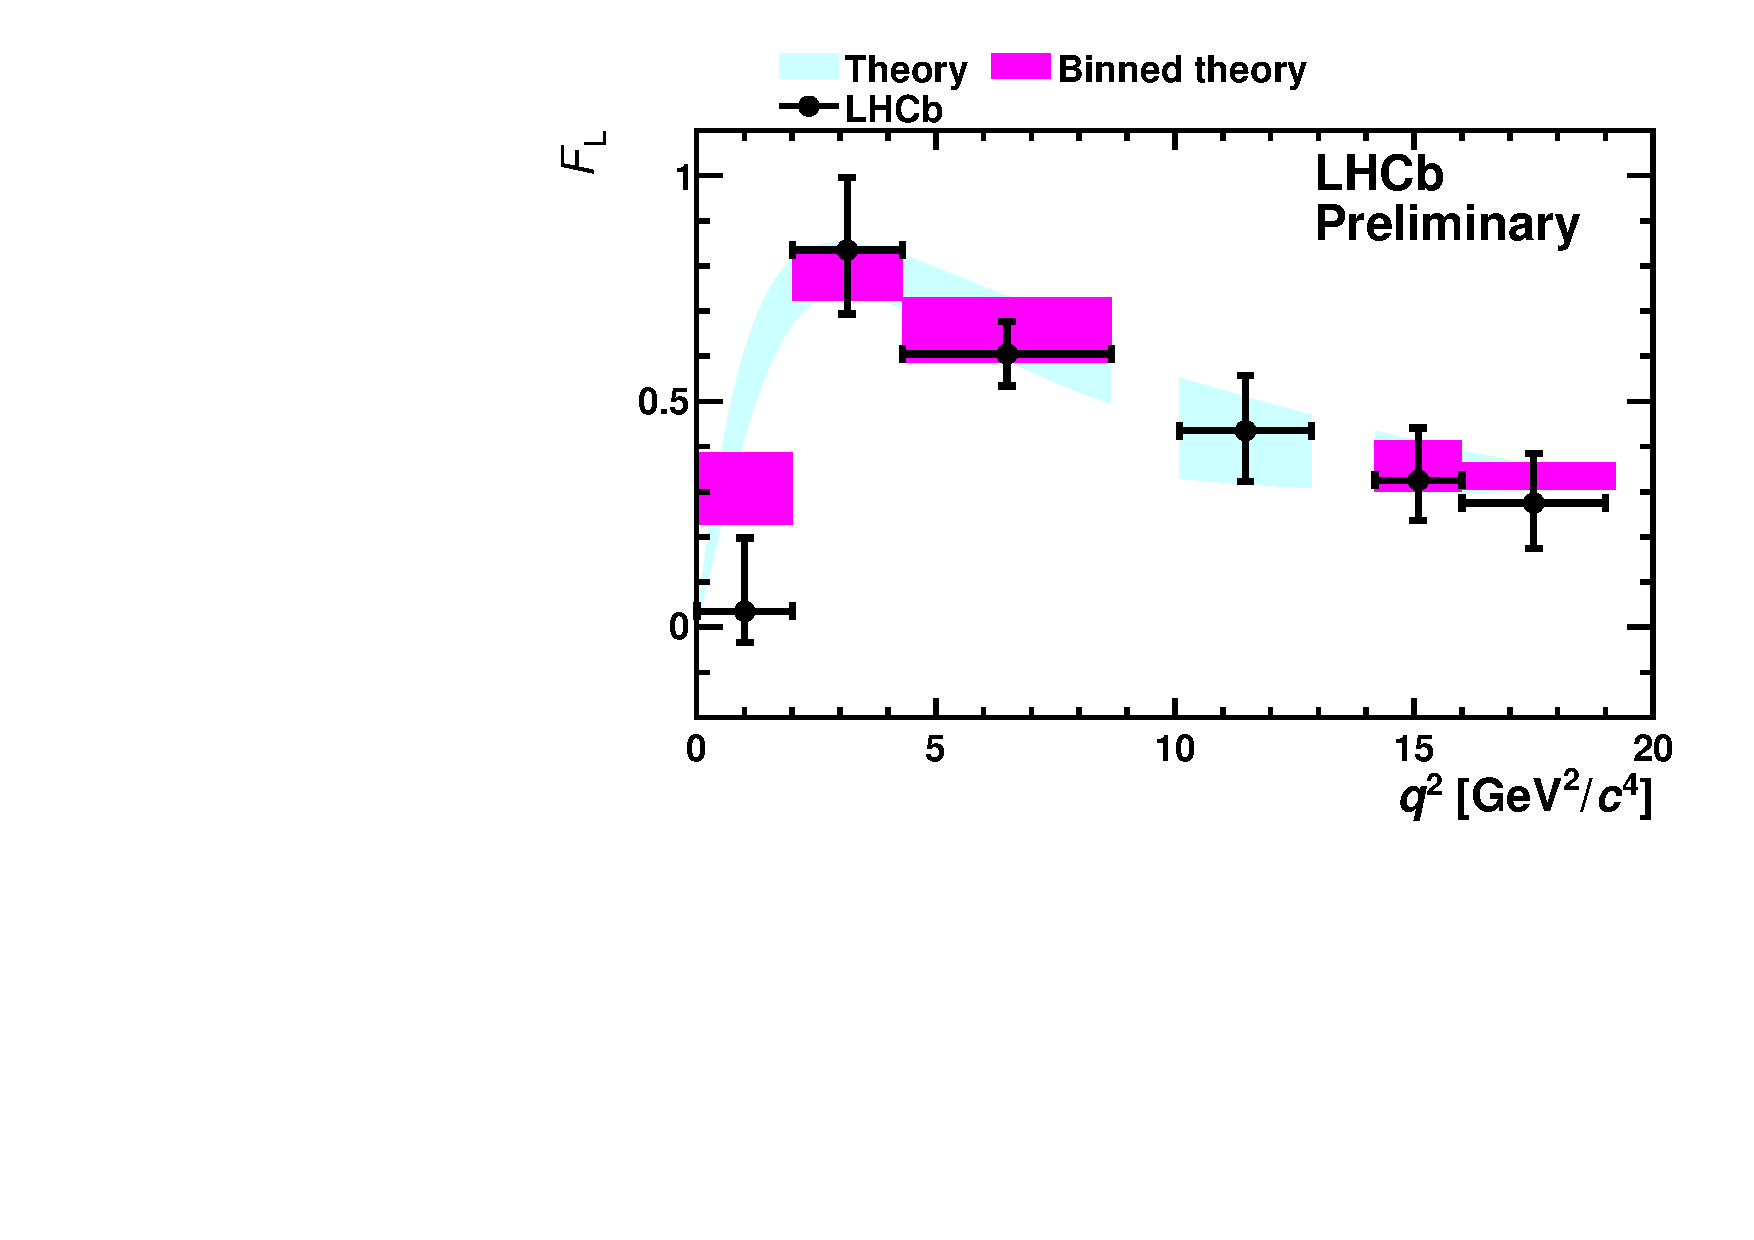
\includegraphics[width=0.52\textwidth]{Fl.pdf}}
   \subfigure{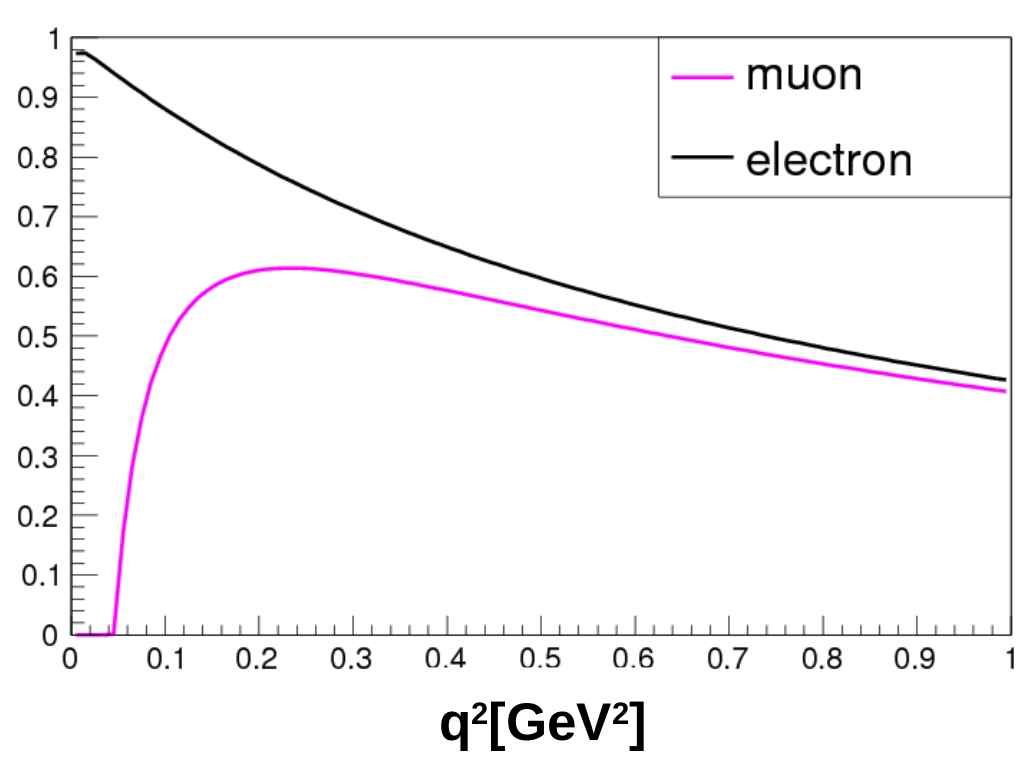
\includegraphics[width=0.47\textwidth]{sensitivity.jpg}}
  \vspace*{-0.5cm}
  \end{center}
  \caption{\textit{The parameter $F_L(q^2)$ (left) and the sensitivity on the parameter $A^{(2)}_T(q^2)$ for muons and electrons (right). $F_L(q^2)$ was determined by analysis of $\Bd \rightarrow K^{*0} \mup \mun$ for different bins of $q^2$.}\cite{mumu}}
  \label{fig:sens}
\end{figure}

\subsection{The lower cut: $q\, > 20\mevcc$}
Although the \BdKstee events at low $q^2$ carry the most information about the photon polarisation a cut of $q\, > 20\mevcc$ has to be performed. At dielectron invariant mass $m(\epem)\approx 0$ the two electrons are nearly collinear and therefore the angle between them is very small. At the limit of $q^2 \rightarrow 0$ the dilepton plane cannot be defined any more and thus the $\Phi$ angle cannot be determined. By experiencing multiple scattering of the electrons in the detector the plane defined by the (\epem) pair is extremely distorted. This leads to a great uncertainty on the $\Phi$ angle which makes these events useless for the angular analysis. Furthermore the measured (\epem) invariant mass is increased due to added opening angle between the electron and the positron due to multiple scattering. \\
To allow for a small uncertainty on the measured $\Phi$ angle a study has been performed on the resolution of the $\Phi$ angle. Figure \ref{fig:phires} shows the resolution of the $\Phi$ angle with respect to the invariant mass of the electron pair. The uncertainty on $\Phi$ drops off exponentially and remains stable from $150 \mevcc$ onwards.\\
The cut of $q\, > 20\mevcc$ was chosen as the $\Phi$ resolution is acceptable at from this value on. This cut also allows to keep a large amount if events with low electron pair invariant mass.
\begin{figure}[ht]
\vspace{-0.4cm}
  \begin{center}
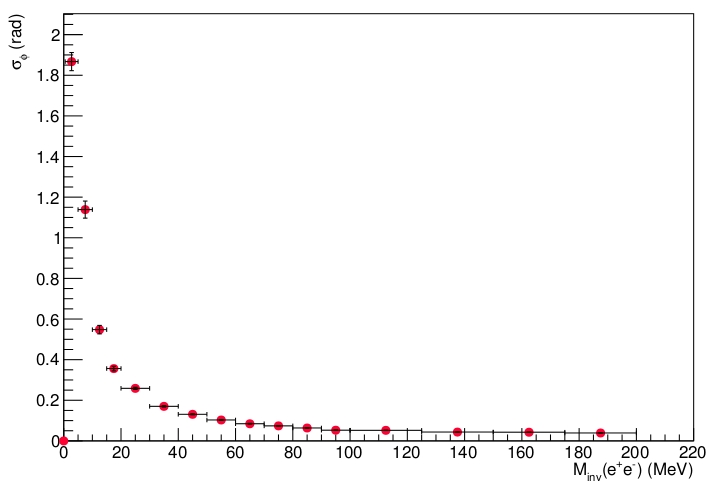
\includegraphics[width=0.5\textwidth]{phires.jpg}
  \vspace*{-0.8cm}
  \end{center}
  \caption{\textit{The resolution of the $\Phi$ angle for different bins of (\epem) invariant mass obtained from \BdKstee Monte Carlo.}}
  \label{fig:phires}
\end{figure}